\documentclass[11pt]{article}

\usepackage[hmargin=1in,vmargin=0.8in]{geometry}
\usepackage{listings}
\usepackage{color}
\usepackage{hyperref}
\usepackage{graphicx}
\usepackage{blindtext}
\usepackage{enumitem}

% For better handling of unicode (Latin characters, anyway)
\IfFileExists{lmodern.sty}{\usepackage{lmodern}}{}
\usepackage[T1]{fontenc}
\usepackage[utf8]{inputenc}

\hypersetup{
    colorlinks=true,
    linkcolor=blue,
    urlcolor=red,
    linktoc=all
}

% bibliographie
\RequirePackage{filecontents}
\begin{filecontents*}{bibliografie.bib}
	@misc{sourceCode,
		author = "PEREIRA Romain",
		title = "Source code",
		howpublished = "\newline\url{https://github.com/rpereira-dev/VoxelEngine.git}",
		note = "\newline The main repository of the project"
	}
\end{filecontents*}

% title setup
\title{How blocks are stored}
\author{Romain PEREIRA}
\date{3rd November 2017}

\renewcommand*\contentsname{Summary}

\begin{document}
	%first page, title, table of content, final result illustration
	\maketitle
	\tableofcontents

	% how to read this document
	\section*{Preamble}
	This file is part of the Voxel Engine project. It is here to document the project, and to explain how the program was conceived.
	It is not a formal scientific paper, but we should try to stick to this style, to make it more readable and interesting.
	Thank you for your attention, have a nice reading.
	\newpage
	
	% abstract: motivation, problem statement, approach, results, conclusions
	\section{Abstract}
	In order to store our voxels, we need a data structure.
	As the software should be dealing with million of blocks, this data structure has to be `memory-friendly', or the whole program won't be able to run.
	That is what `Terrain' are: a data structure.
	\newline
	The approach assumes that we need to store in RAM informations about each loaded blocks, not less, not more.
	These informatons are numerous: block behaviour (transparency, liquid, density, light emitter...), block rendering (lighting, mesh
	\newline
	Final results were definetly acceptable: the programs need 4 bytes per block.
	On a 1GB virtual machine, this would mean being able to fastly access more than 250 000 000 blocks.
	(which is the number of water drop on a $20m^3$ container.)
	\begin{figure}[!h]
		\begin{center}
			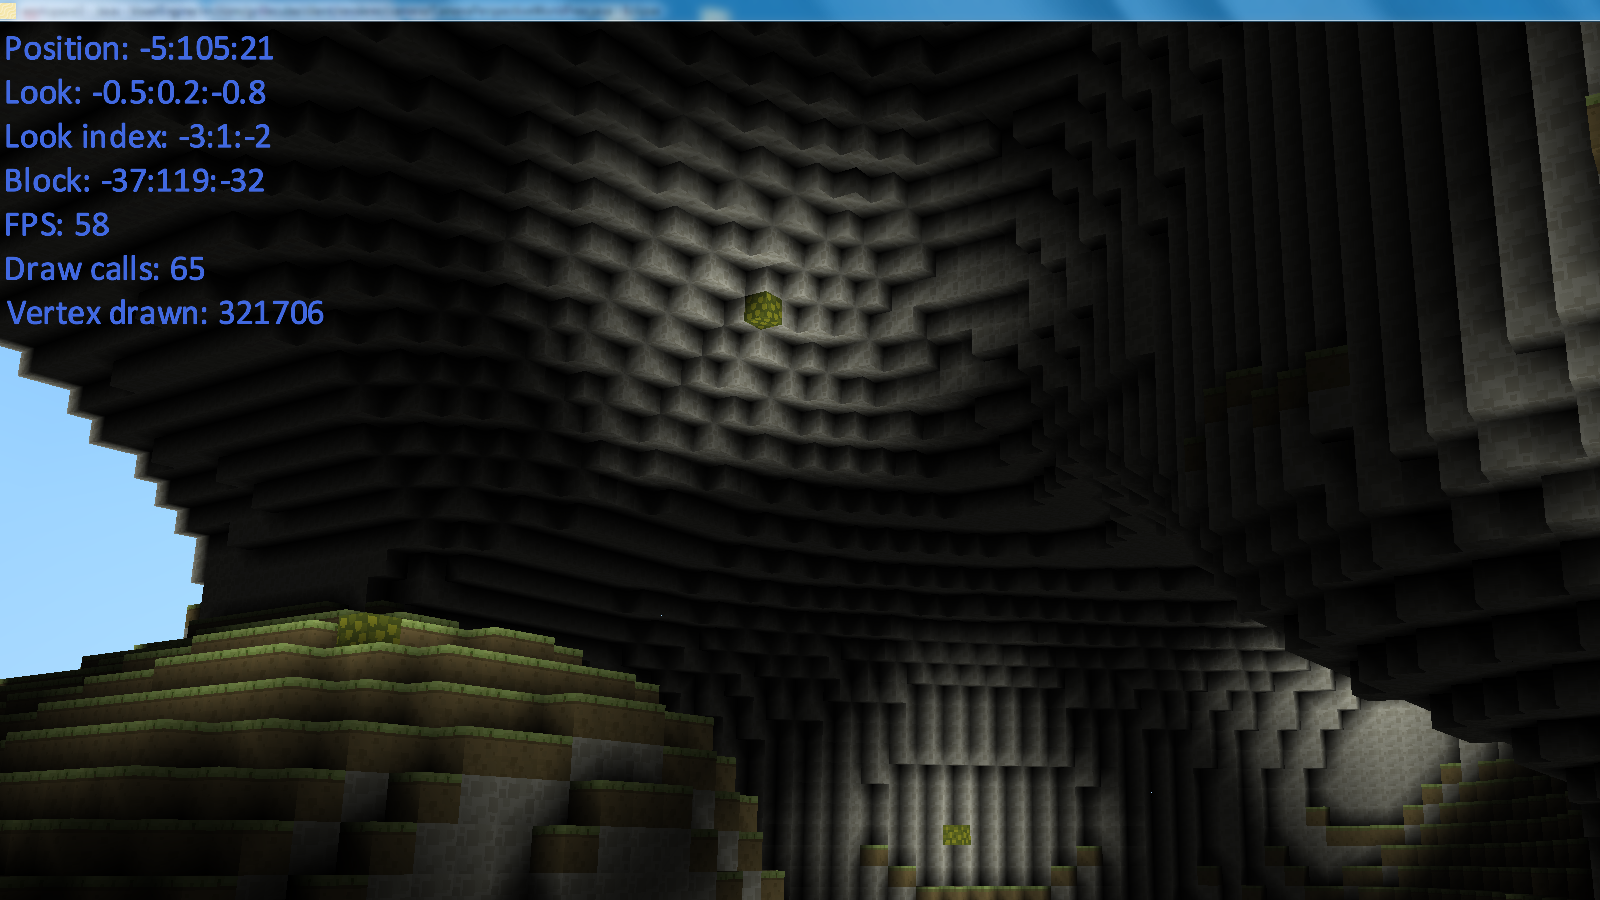
\includegraphics[width=0.6\textwidth,height=0.6\textheight,keepaspectratio]{./assets/title.png}
		\end{center}
		\caption{\textit{Illustration of the final result}}
		\label{Title illustration}
	\end{figure}
	\newpage

	% introduction
	\section{Introduction}
	\newpage

	% body
	\section{Materials and methods}
		\subsection{Memory representation}
			\subsubsection{Naive approach}
				Each blocks need attributes: textures, densities, light value, materials, amount of water...											\newline
				If we store each blocks in it own instance with these attributes, the amount of memory per block (in bytes) would be:
				\[S_{b}=pointer + textures + density + light value + ... >= 40 \textrm{ bytes}\]
				where:
				\begin{itemize}
					\item pointer: pointer to the block memory address (8 bytes)
					\item textures: textures integer id for each block faces (6 faces * 4 bytes per faces)
					\item density: float 4 bytes
					\item light value: float 4 bytes
					\item [...] and many other imagineable attributes.
				\end{itemize}
				However, many blocks \underline{shares constants attributes}. (each `stone' block have the same density for example)
				\newline
				Moreover, Most of the block (> 80\% of them) will be dirt, stone, leaves...
				These blocks have many shared constants attributes. So, \underline{instancing is the key}.
				\newline
			
			\subsubsection{Instancing}
				Let us seperate blocks in two categories: the one that don't need their own instance A), and the one who need it own 							instances B).
				\newline
				\newline
				In category A, we find for instance: dirt, stone, leaves, logs, plants...
				\newline
				\newline
				Each of these blocks need: 1 integer (which will be codded on 2 bytes in practice), representing the 
				In category B, we find liquids (each blocks has it own amount of liquids), or any dynamic blocks that need it own `per block' 						attributes.
				\newline
				\underline{NB:} B inherits A
			
			\subsubsection{Terrain}
				A `Terrain' simply is a $u*v*w$ 4 bytes-array, which hold blocks. Moreover, it contains a 3 integers `world-relative'
				index $(ix, iy, z)$, so we can change from `Terrain' basis coordinate system to global `World' basis.
				\newline
				TODO: 2D terrain scheme
				\newline
				\newline
				The memory usage of a terrain (which can hold $u*v*w$ block from category A)) is:
				\[S_{t}=4 * u * v * w + o(u*v*w)\]
				where:
				\begin{itemize}
					\item $o(u*v*w)$ is the size of every per-Terrain attributes
				\end{itemize}
				and so, per block:
				\newline
				\[S_{b}=4 + o(1) \simeq4.1 \textrm{ bytes (in practice)}\]							
				\newline
				\newline
				To optimize memory access (reading and writting), the 3 dimensionals array was flattened, see:
				\newline
				https://stackoverflow.com/questions/2512082/java-multi-dimensional-array-vs-one-dimensional				
		\subsection{sub section 2}
	\newpage
	
	% general conclusion, performances, what can be improved ...
	\section{General conclusion}
	\newpage
	
	% bibliography
	\nocite{*}
	\bibliographystyle{amsplain}
	\bibliography{bibliografie}

\end{document}